\documentclass[tikz,border=7pt]{standalone}
\usepackage{amsmath}
\usepackage{pgfplots}
\pgfplotsset{compat=1.18}

\definecolor{ink}{HTML}{21352F}
\definecolor{teal}{HTML}{087F7B}
\definecolor{rose}{HTML}{B65A62}
\definecolor{gold}{HTML}{C58B2A}

\begin{document}
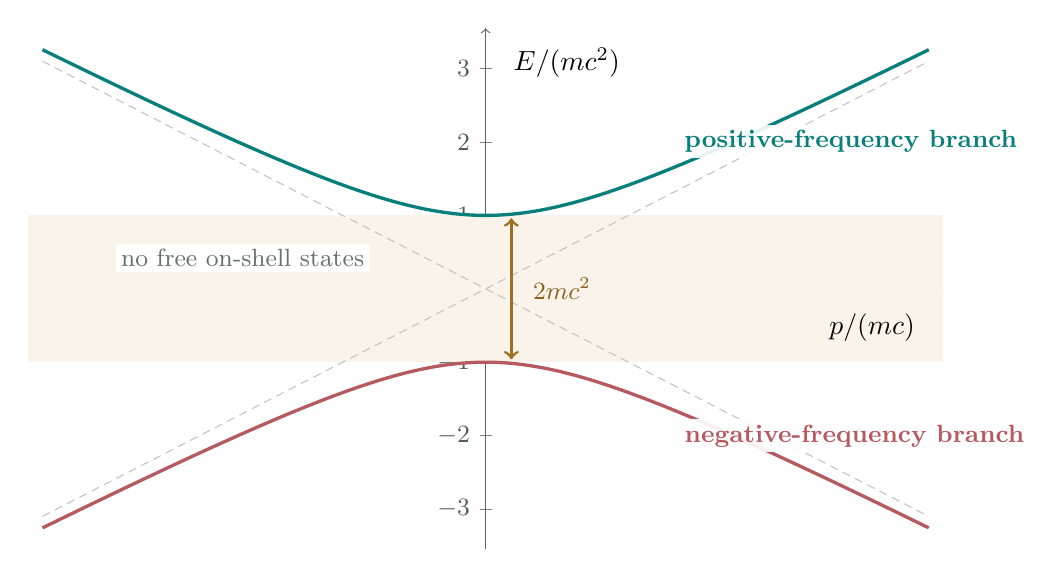
\begin{tikzpicture}[font=\sffamily]
\begin{axis}[
  width=13.2cm,
  height=8.2cm,
  xmin=-3.2,
  xmax=3.2,
  ymin=-3.55,
  ymax=3.55,
  axis lines=middle,
  axis line style={draw=ink!75,->},
  xlabel={$p/(mc)$},
  ylabel={$E/(mc^2)$},
  xlabel style={at={(axis description cs:0.98,0.47)},anchor=north east},
  ylabel style={at={(axis description cs:0.52,0.98)},anchor=north west},
  xtick={-3,-2,-1,0,1,2,3},
  ytick={-3,-2,-1,1,2,3},
  tick label style={font=\small,text=ink!80},
  clip=false
]
  \path[fill=gold!10]
    (axis cs:-3.2,-1) rectangle (axis cs:3.2,1);

  \addplot[teal,very thick,domain=-3.1:3.1,samples=180]
    {sqrt(1+x^2)};
  \addplot[rose,very thick,domain=-3.1:3.1,samples=180]
    {-sqrt(1+x^2)};

  \addplot[ink!28,densely dashed,domain=-3.1:3.1,samples=3]
    {abs(x)};
  \addplot[ink!28,densely dashed,domain=-3.1:3.1,samples=3]
    {-abs(x)};

  \node[teal,anchor=south west,font=\small\bfseries,
        fill=white,fill opacity=0.9,text opacity=1,inner sep=2pt]
    at (axis cs:1.35,1.77) {positive-frequency branch};
  \node[rose,anchor=north west,font=\small\bfseries,
        fill=white,fill opacity=0.9,text opacity=1,inner sep=2pt]
    at (axis cs:1.35,-1.77) {negative-frequency branch};

  \draw[gold!80!black,<->,line width=1pt]
    (axis cs:0.18,-0.96) -- (axis cs:0.18,0.96)
    node[midway,right=4pt,font=\small,text=gold!70!black]
    {$2mc^2$};

  \node[font=\small,text=ink!70,fill=white,inner sep=2pt]
    at (axis cs:-1.7,0.42) {no free on-shell states};
\end{axis}
\end{tikzpicture}
\end{document}
